\clearpage
\section{Suns-Voc editor}
The Suns-Voc plugin can be used to calculate how open circuit voltage changes as a function of light intensity.  This can be useful for understanding tail slope and disorder in devices.  A picture of the suns-voc editor window can be seen below in figure \ref{fig:sunsvoceditor}.  The window can be used to set the start and stop light intensity. The Suns-Voc applies the voltage to the contact that is labelled \emph{Change}.

\begin{figure}[H]
\centering
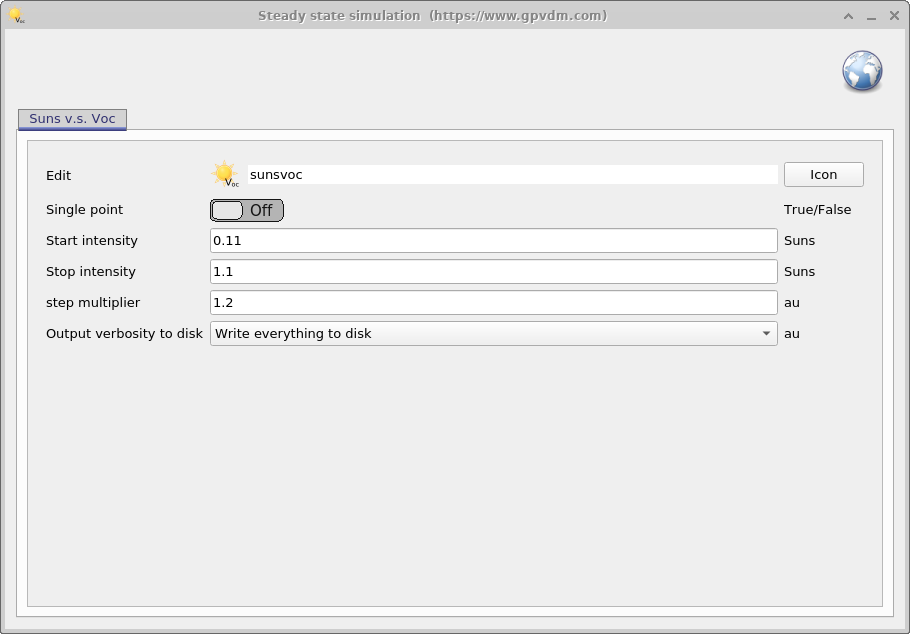
\includegraphics[width=0.7\textwidth,height=0.5\textwidth]{./images/sim_editors/suns_voc_editor.png}
\caption{The suns-voc editor window}
\label{fig:sunsvoceditor}
\end{figure}


\subsection{Outputs}

\begin{table}[H]
\begin{center}
\begin{tabular}{ |c|c| } 
 \hline
	File name 			& 	Description  \\ 
 \hline
	suns\_voc.csv 		&	Suns v.s. Voc curve \\ 
	suns\_Q.csv 		&	Suns v.s. Charge density\\ 
	suns\_mu.csv 		&	Suns v.s. average charge carrier mobility\\
	suns\_tau.csv 		&	Suns v.s. recombination constant tau \\ 
	Q\_Qtau.csv 		&	Charge density v.s. recombination constant tau \\
	Q\_mu.csv 			&	Charge density v.s. charge carrier mobility\\
	Q\_kbi.csv 			&	Charge density v.s. recombination prefactor kbi\\
	Q\_trap\_filling.csv &	Charge density v.s. fraction of filled traps\\
	V\_mu.csv 			&	Voc v.s. average charge carrier mobility\\
 \hline
\end{tabular}
\caption{Files produced by the Suns-Voc simulation}
\label{tab:suns_voc_output}
\end{center}
\end{table}

